%%%%%%%%%%%%%%%%%%%%%%%%%%%%%%%%%%%%%%%%%
% Beamer Presentation
% LaTeX Template
% Version 1.0 (10/11/12)
%
% This template has been downloaded from:
% http://www.LaTeXTemplates.com
%
% License:
% CC BY-NC-SA 3.0 (http://creativecommons.org/licenses/by-nc-sa/3.0/)
%
%%%%%%%%%%%%%%%%%%%%%%%%%%%%%%%%%%%%%%%%%

%----------------------------------------------------------------------------------------
%	PACKAGES AND THEMES
%----------------------------------------------------------------------------------------

\documentclass[UTF8,aspectratio=169,14pt]{ctexbeamer}

\usepackage{hyperref}
\hypersetup{
	colorlinks=true,
	linkcolor=red,
	anchorcolor=blue,
	citecolor=green
}

\mode<presentation> {
	
	% The Beamer class comes with a number of default slide themes
	% which change the colors and layouts of slides. Below this is a list
	% of all the themes, uncomment each in turn to see what they look like.
	
	%\usetheme{default}
	%\usetheme{AnnArbor}
	%\usetheme{Antibes}
	%\usetheme{Bergen}
	%\usetheme{Berkeley}
	%\usetheme{Berlin}
	%\usetheme{Boadilla}
	%\usetheme{CambridgeUS}
	%\usetheme{Copenhagen}
	%\usetheme{Darmstadt}
	%\usetheme{Dresden}
	%\usetheme{Frankfurt}
	%\usetheme{Goettingen}
	%\usetheme{Hannover}
	%\usetheme{Ilmenau}
	%\usetheme{JuanLesPins}
	%\usetheme{Luebeck}
	\usetheme{Madrid}
	%\usetheme{Malmoe}
	%\usetheme{Marburg}
	%\usetheme{Montpellier}
	%\usetheme{PaloAlto}
	%\usetheme{Pittsburgh}
	%\usetheme{Rochester}
	%\usetheme{Singapore}
	%\usetheme{Szeged}
	%\usetheme{Warsaw}
	
	% As well as themes, the Beamer class has a number of color themes
	% for any slide theme. Uncomment each of these in turn to see how it
	% changes the colors of your current slide theme.
	
	%\usecolortheme{albatross}
	%\usecolortheme{beaver}
	%\usecolortheme{beetle}
	%\usecolortheme{crane}
	%\usecolortheme{dolphin}
	%\usecolortheme{dove}
	%\usecolortheme{fly}
	%\usecolortheme{lily}
	%\usecolortheme{orchid}
	%\usecolortheme{rose}
	%\usecolortheme{seagull}
	%\usecolortheme{seahorse}
	%\usecolortheme{whale}
	%\usecolortheme{wolverine}
	
	%\setbeamertemplate{footline} % To remove the footer line in all slides uncomment this line
	%\setbeamertemplate{footline}[page number] % To replace the footer line in all slides with a simple slide count uncomment this line
	
	%\setbeamertemplate{navigation symbols}{} % To remove the navigation symbols from the bottom of all slides uncomment this line
}

\usepackage{graphicx} % Allows including images
\graphicspath{{./figs/}}
\usepackage{booktabs} % Allows the use of \toprule, \midrule and \bottomrule in tables
\usepackage{longtable}
\usepackage{listings}
\usepackage{xcolor}
\lstset{numbers=left, %设置行号位置
	numberstyle=\tiny, %设置行号大小
	keywordstyle=\color{blue}, %设置关键字颜色
	commentstyle=\color[cmyk]{1,0,1,0}, %设置注释颜色
	frame=single, %设置边框格式
	escapeinside=``, %逃逸字符(1左面的键),用于显示中文
	%breaklines, %自动折行
	extendedchars=false, %解决代码跨页时,章节标题,页眉等汉字不显示的问题
	xleftmargin=2em,xrightmargin=2em, aboveskip=1em, %设置边距
	tabsize=4, %设置tab空格数
	showspaces=false %不显示空格
}
% Fonts
% \usepackage{libertine}
% \setmonofont{Courier}
\setCJKsansfont[ItalicFont=Noto Serif CJK SC Black, BoldFont=Noto Sans CJK SC Black]{Noto Sans CJK SC}


%----------------------------------------------------------------------------------------
%	TITLE PAGE
%----------------------------------------------------------------------------------------

\title[第2讲]{第2讲 :中断、异常与系统调用 } % The short title appears at the bottom of every slide, the full title is only on the title page
\subtitle{第三节:kernel mode 操作系统}
\author{向勇、陈渝、李国良} % Your name
\institute[清华大学] % Your institution as it will appear on the bottom of every slide, may be shorthand to save space
{
清华大学计算机系 \\ % Your institution for the title page
\medskip
\textit{xyong,yuchen@tsinghua.edu.cn} % Your email address
}
\date{\today} % Date, can be changed to a custom date

\begin{document}

\begin{frame}
\titlepage % Print the title page as the first slide
\end{frame}

%\begin{frame}
%\frametitle{提纲} % Table of contents slide, comment this block out to remove it
%\tableofcontents % Throughout your presentation, if you choose to use \section{} and \subsection{} commands, these will automatically be printed on this slide as an overview of your presentation
%\end{frame}

%----------------------------------------------------------------------------------------
%	PRESENTATION SLIDES
%----------------------------------------------------------------------------------------

%------------------------------------------------
%\section{第四节:RISC-V CPU启动}% Sections can be created in order to organize your presentation into discrete blocks, all sections and subsections are automatically printed in the table of contents as an overview of the talk
%------------------------------------------------

%\subsection{高级语言编译到机器指令} % A subsection can be created just before a set of slides with a common theme to further break down your presentation into chunks
%\subsection{理解stack}


%\begin{frame}
%	\frametitle{RISC-V CPU}
%	\framesubtitle{系统编程语言}

%\begin{figure}
%\centering
%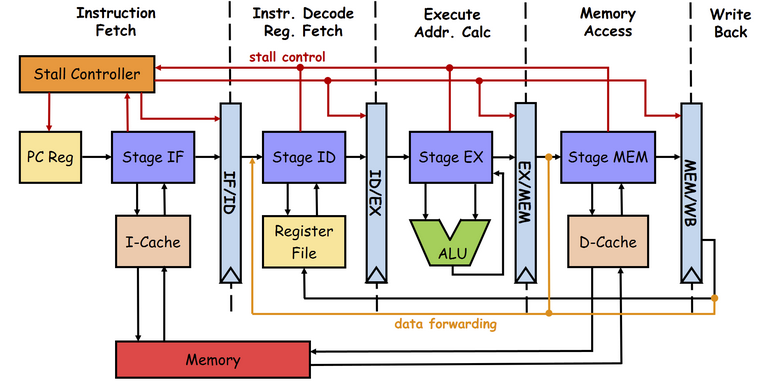
\includegraphics[width=0.8\linewidth]{five-stage-rv}

%\caption{5级流水线RISC-V CPU}
%\end{figure}

%\end{frame}
%------------------------------------------------
\begin{frame}
    \frametitle{内容简介}
    \begin{itemize}
        \item 回顾特权级切换
        \item 用户态应用程序:控制逻辑,地址空间,系统调用
        \item kernel-mode OS:启动,初始化,创建执行应用,系统调用服务
    \end{itemize}
\end{frame}

%------------------------------------------------
\begin{frame}
	\frametitle{kernel mode OS: RISC-V CPU特权级切换}
%	\framesubtitle{QEMU}
%\begin{figure}
	\centering
	
\includegraphics[width=0.2\linewidth]{qemu}
	
%	\caption{QEMU for RISC-V CPU}
%\end{figure}	
%	\begin{itemize}
%		
%		\item RISC-V
%		\begin{itemize}
%			\item CPU: RV64 ISA with MMU/TLB
%			\item MEM: ROM, RAM,IO-MEM, etc
%			\item I/O:Timer, UART
%			\item Interrupt: PLIC(Platform-Level Interrupt Controller) -- Device
%			\item Interrupt: CLINT(Core Local Interruptor) -- Timer, IPI 
%		\end{itemize}
%
%	\end{itemize}	
\begin{figure}
	\centering
    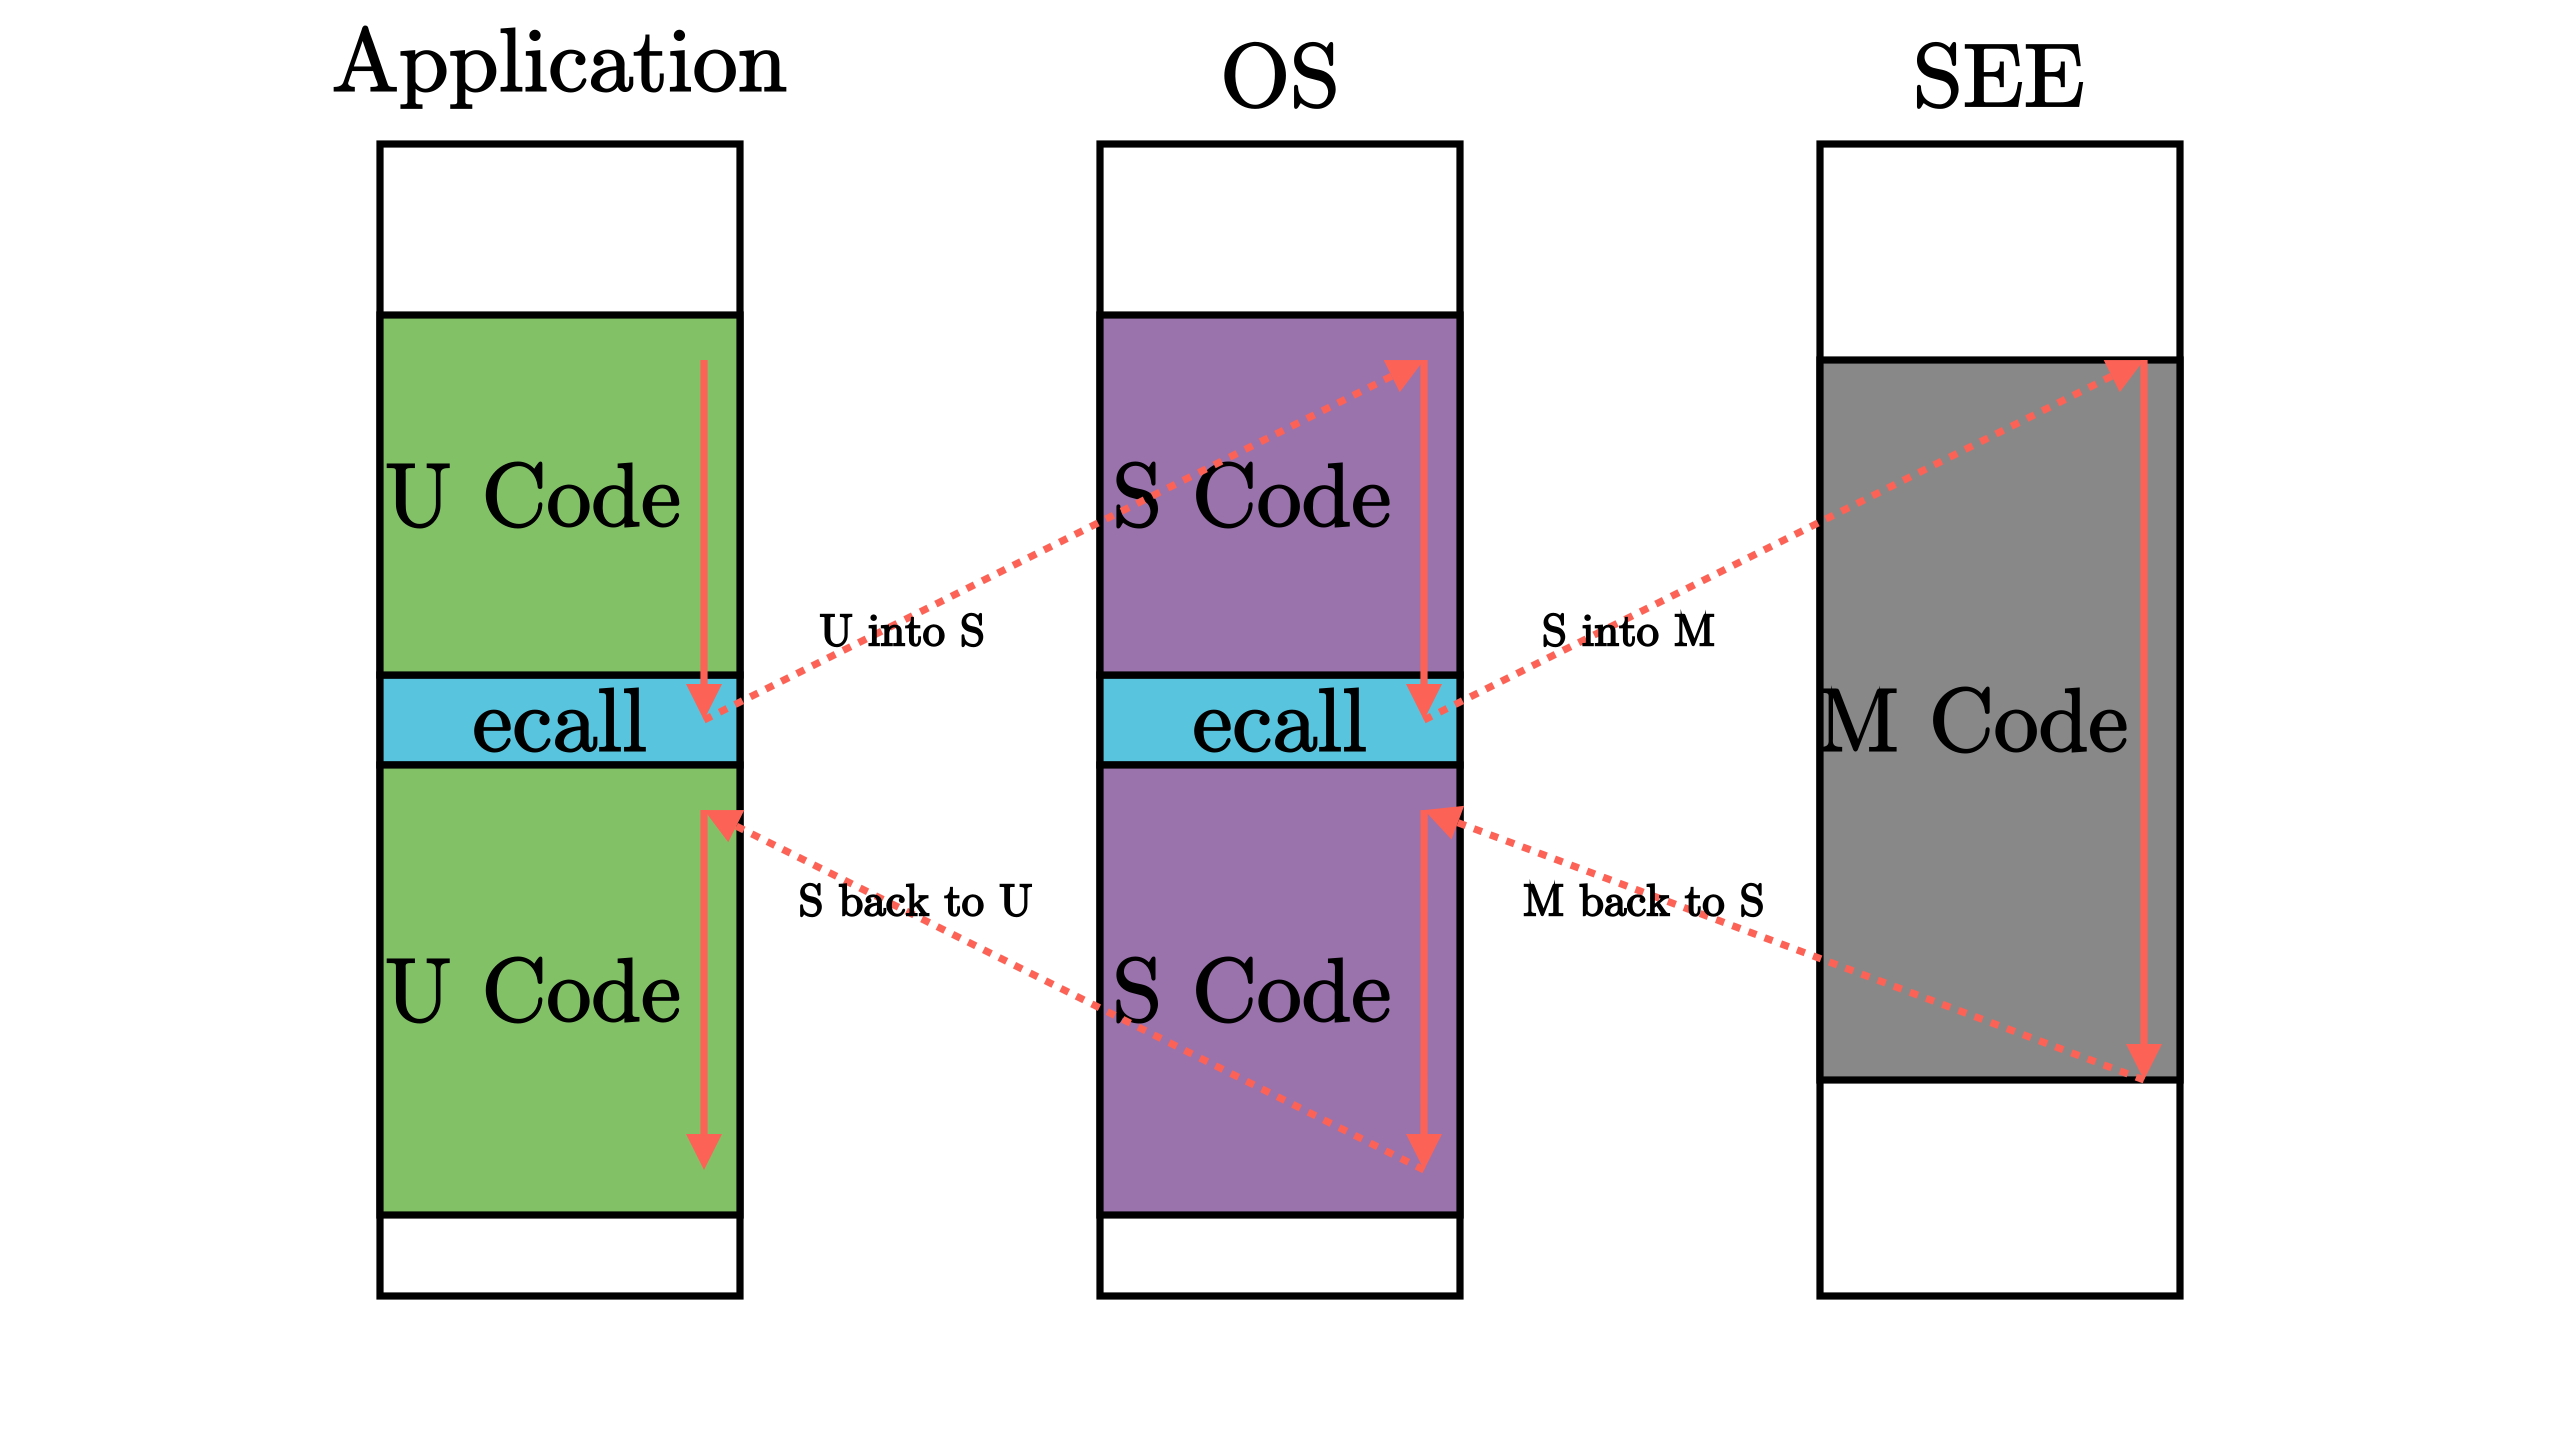
\includegraphics[width=0.6\linewidth]{EnvironmentCallFlow}
    	\caption{RISC-V CPU特权级切换}
    \end{figure}	
\end{frame}

%------------------------------------------------

\begin{frame}
    
    \frametitle{kernel mode OS: U-Mode 应用程序}
    U-Mode 应用程序
    \centering
    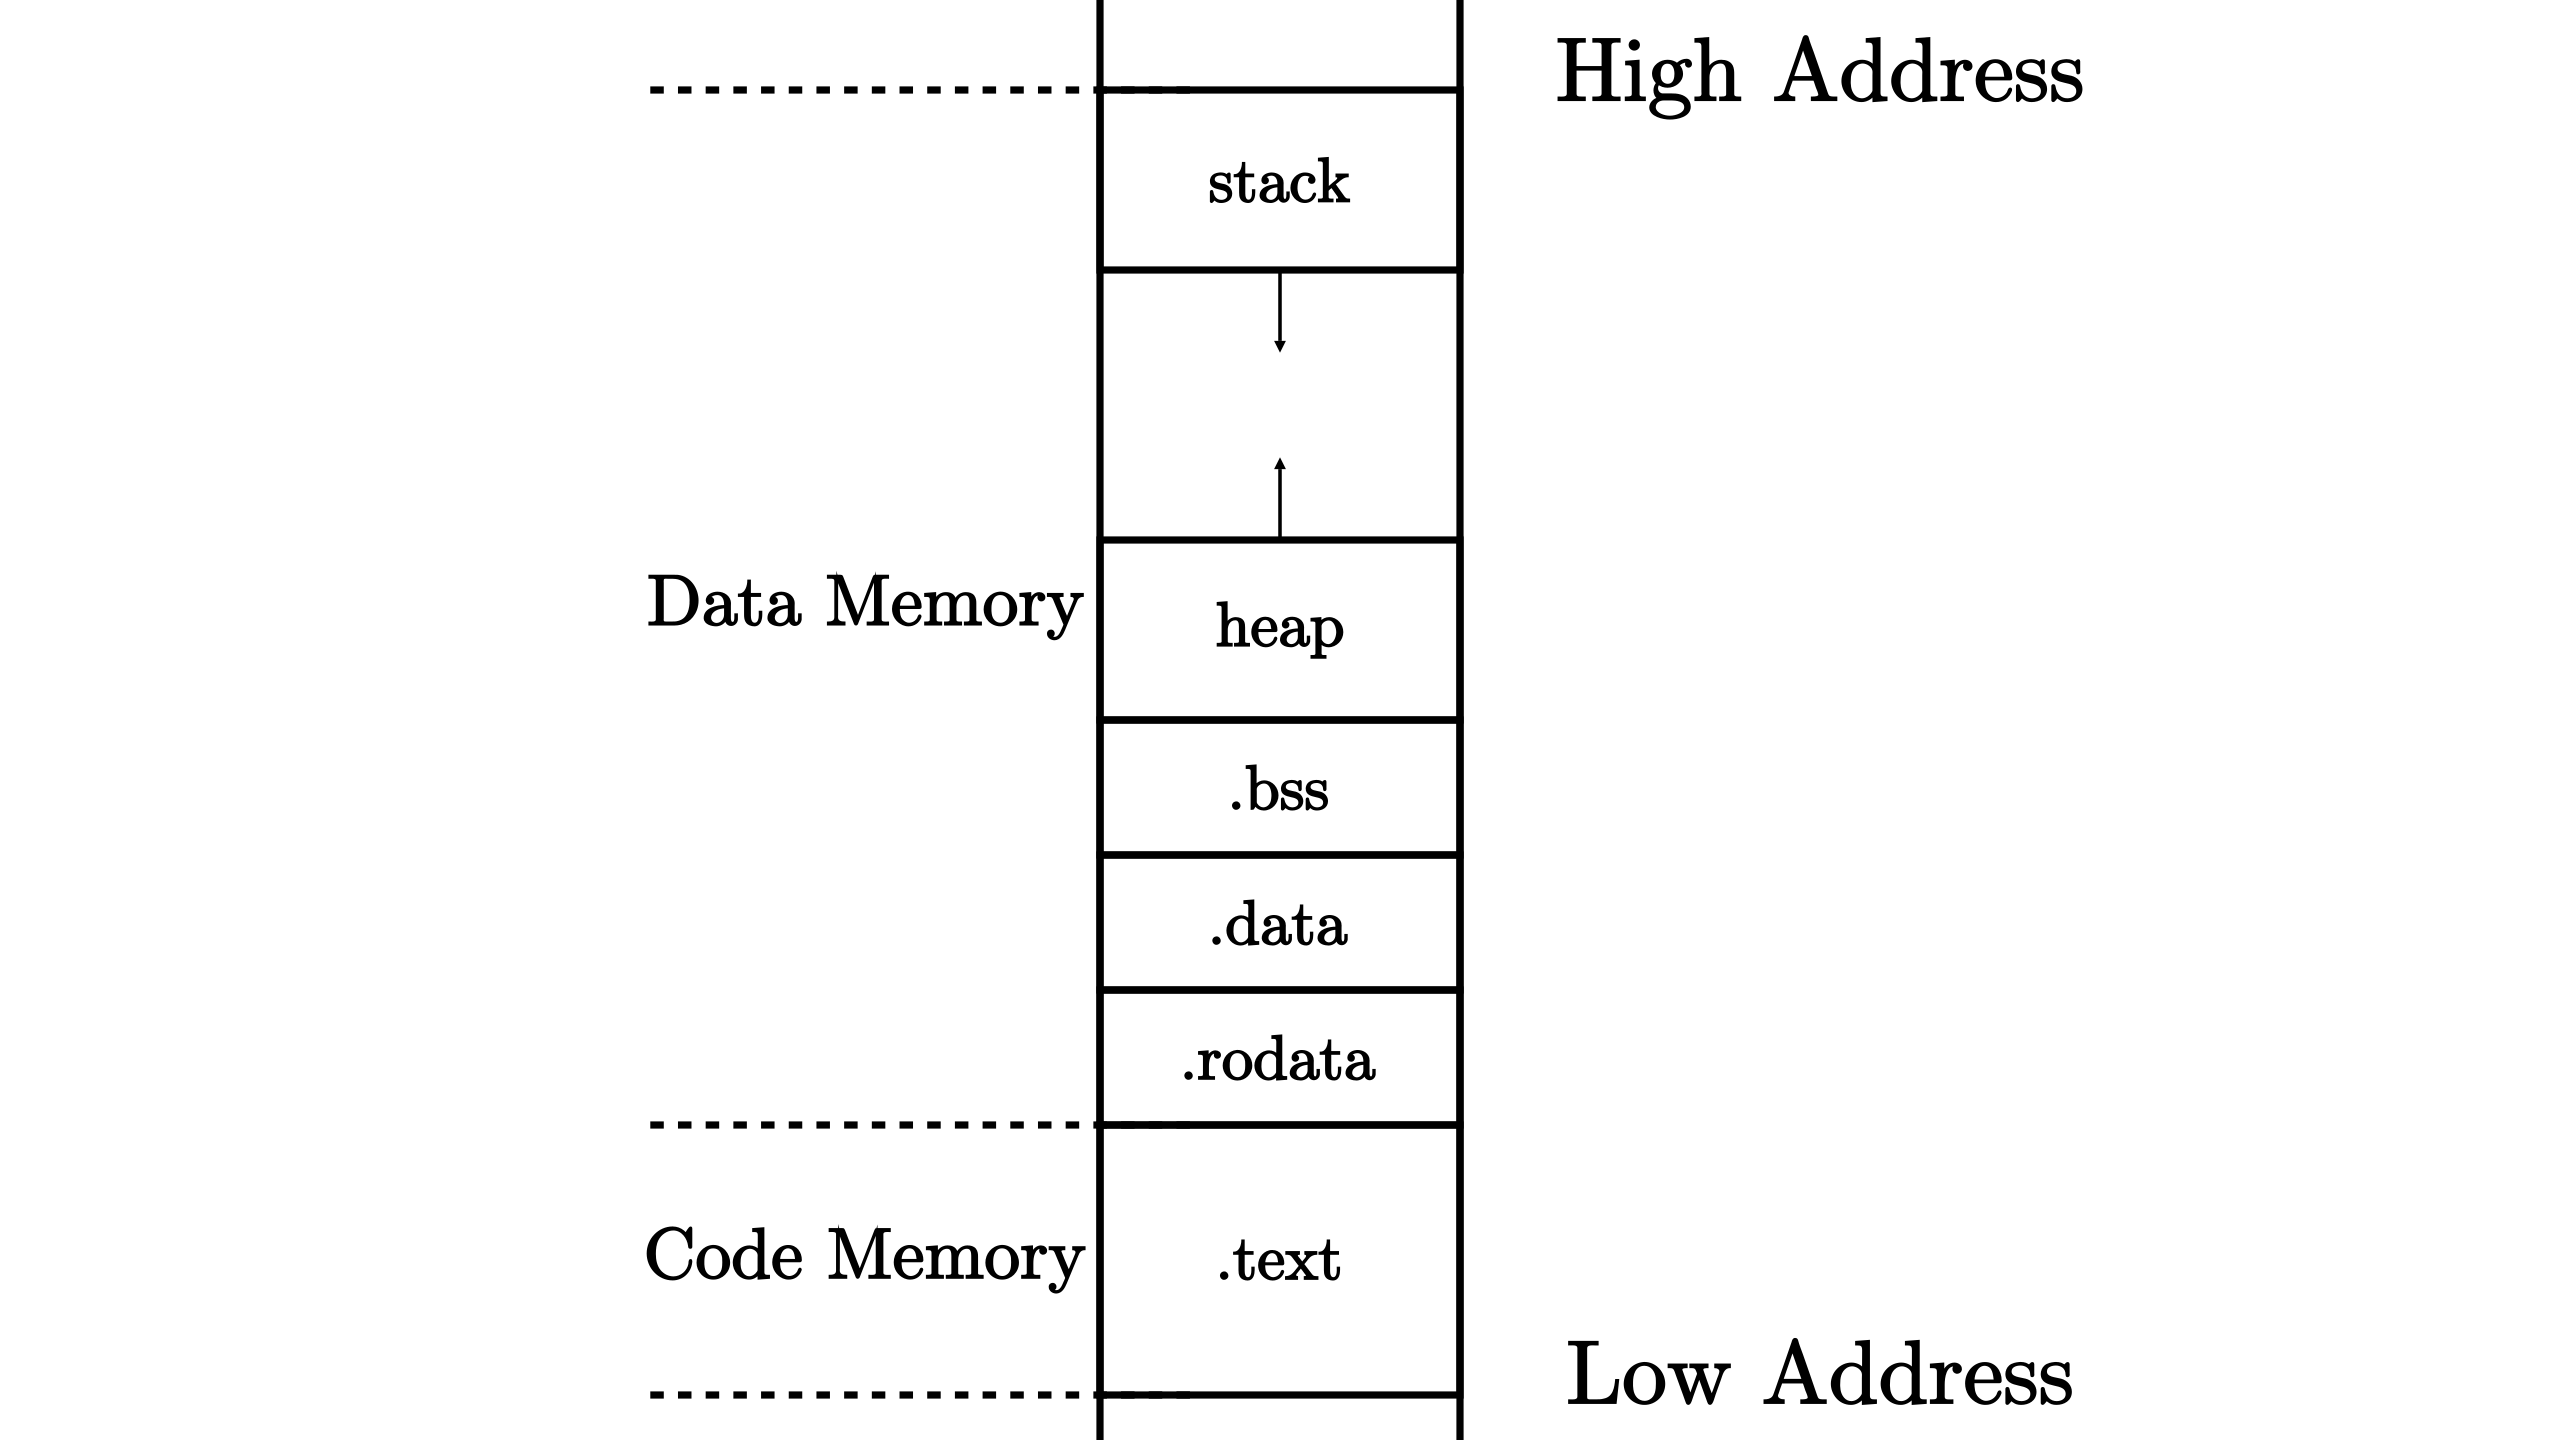
\includegraphics[width=0.8\linewidth]{app-mem-layout}
    
\end{frame}

%------------------------------------------------
\begin{frame}
	\frametitle{kernel mode OS: U-Mode 应用程序}
%	\framesubtitle{QEMU}
%	\centering
%	
\includegraphics[width=0.2\linewidth]{qemu}	
%	\begin{itemize}
%		
%		\item RISC-V CPU 启动过程
%		\begin{itemize}
%			\item 初始化CPU/Regs	
%			\item 初始化内存
%			\item 初始化基本外设
%			\item 执行ROM中固化的代码
%		\end{itemize}
%		\item 出处: \href{https://github.com/qemu/qemu}{https://github.com/qemu/qemu}
%		
%	\end{itemize}	

应用程序的执行环境的建立是编译器,库和OS的共同努力
	\begin{figure}
        \centering
        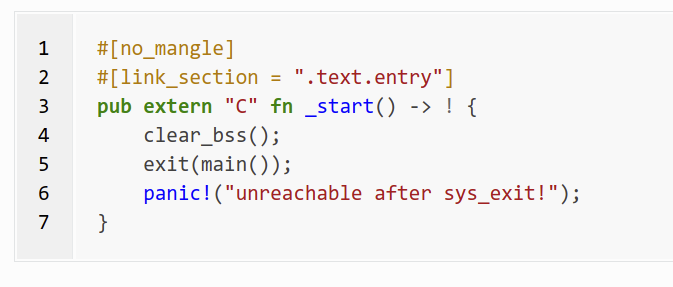
\includegraphics[width=0.8\linewidth]{umode-app}
        \caption{U-Mode 应用程序的执行环境}
    \end{figure}
\end{frame}
%------------------------------------------------

\begin{frame}
    \frametitle{kernel mode OS: U-Mode 应用程序内存布局}
    %	\framesubtitle{QEMU}
    %	\centering
    %	
\includegraphics[width=0.2\linewidth]{qemu}	
    	\begin{itemize}
    		
    		\item 将程序的起始地址调整为某个地址,程序都会被加载到这个地址上运行
    		
    		\item 将 \_start 所在的 .text.entry 放在整个程序的开头,也就是说只要在加载之后跳转到 0x80040000 就已经进入了 用户库的入口点,完成初始化
            \item 提供了执行文件的 .bss 段的起始和终止地址,方便 clear\_bss 函数使用
            \item 提供栈(stack)的地址空间
    		
    	\end{itemize}	
    \begin{figure}
        \centering
        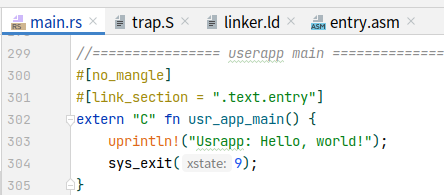
\includegraphics[width=0.5\linewidth]{userapp-main}
        \caption{U-Mode 应用程序}
    \end{figure}
\end{frame}

\begin{frame}
    \frametitle{kernel mode OS: U-Mode 应用程序系统调用}
    %	\framesubtitle{QEMU}
    %	\centering
    %	
\includegraphics[width=0.2\linewidth]{qemu}	
%    \begin{itemize}
%        
%        \item 将程序的起始地址调整为 0x80040000 ,程序都会被加载到这个地址上运行
%        
%        \item 将 \_start 所在的 .text.entry 放在整个程序的开头,也就是说只要在加载之后跳转到 0x80040000 就已经进入了 用户库的入口点,完成初始化
%        \item 提供了执行文件的 .bss 段的起始和终止地址,方便 clear\_bss 函数使用
%        
%    \end{itemize}	
    \begin{figure}
        \centering
        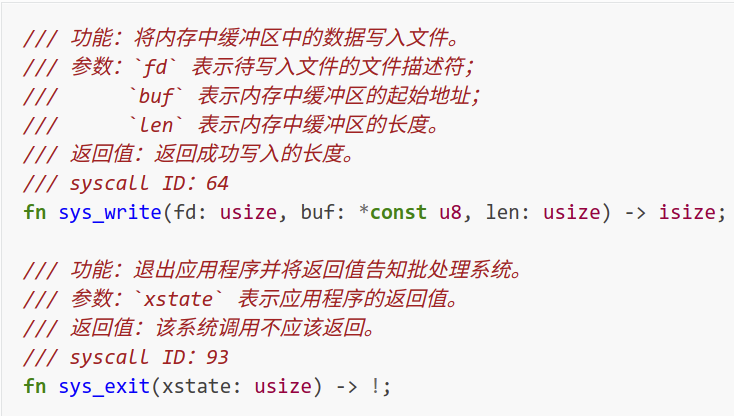
\includegraphics[width=0.6\linewidth]{umode-app-syscall}
        \caption{U-Mode 应用程序系统调用}
    \end{figure}
\end{frame}
%------------------------------------------------
\begin{frame}
    \frametitle{kernel mode OS: U-Mode 应用程序系统调用实现}
    %	\framesubtitle{QEMU}
    %	\centering
    %	
\includegraphics[width=0.2\linewidth]{qemu}	
        \begin{itemize}
            
            \item 约定寄存器 a0-a6 保存系统调用的参数, a0-a1 保存系统调用的返回值。寄存器 a7 用来传递 syscall ID
            
        \end{itemize}	
    \begin{figure}
        \centering
        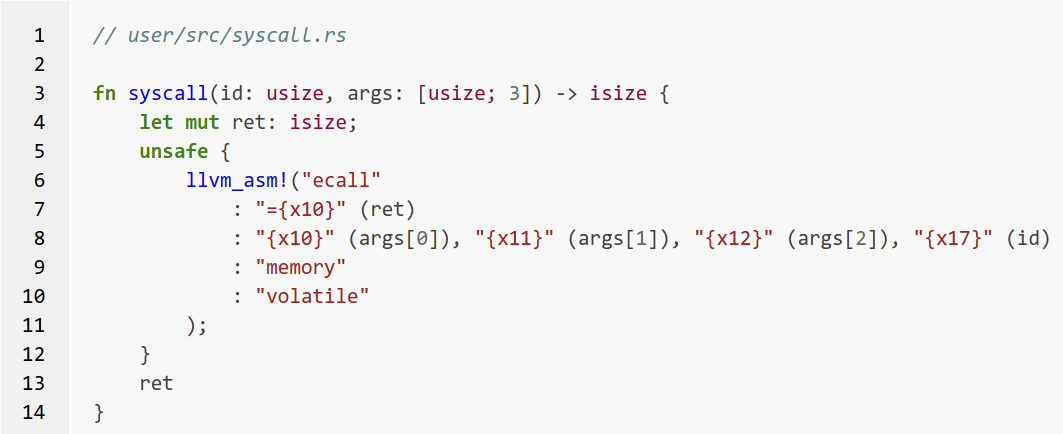
\includegraphics[width=0.8\linewidth]{umode-app-syscall-impl}
        \caption{U-Mode 应用程序系统调用实现}
    \end{figure}
\end{frame}
%------------------------------------------------
%------------------------------------------------
\begin{frame}
    \frametitle{kernel mode OS: 内核实现:启动}
    %	\framesubtitle{QEMU}
    %	\centering
    %	
\includegraphics[width=0.2\linewidth]{qemu}	
    \begin{itemize}
        
        \item 启动:设置栈,跳转到rust\_main函数
        
    \end{itemize}	
    \begin{figure}
        \centering
        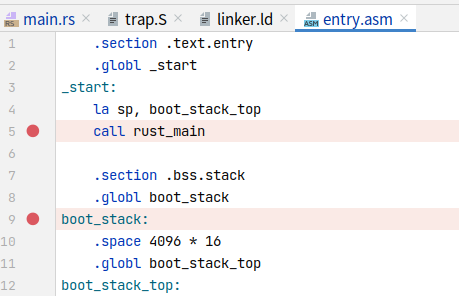
\includegraphics[width=0.6\linewidth]{os-entry}
        \caption{内核启动}
    \end{figure}
\end{frame}

%------------------------------------------------
\begin{frame}
    \frametitle{kernel mode OS: 内核实现:初始化}
    %	\framesubtitle{QEMU}
    %	\centering
    %	
\includegraphics[width=0.2\linewidth]{qemu}	
    初始化:
    \begin{itemize}
        
        \item 初始化系统调用处理(也可被中断和异常处理共享)
        \item 初始化和创建应用程序执行环境
        \item 特权级切换并返回到应用程序的环境中去执行
        
    \end{itemize}	
%    \begin{figure}
        \centering
        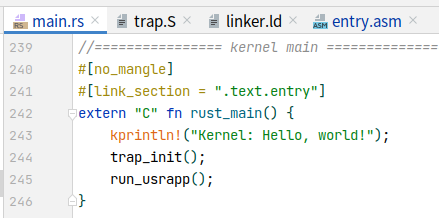
\includegraphics[width=0.6\linewidth]{os-init}
%        \caption{内核初始化}
%    \end{figure}
\end{frame}
%------------------------------------------------

%------------------------------------------------
\begin{frame}
    \frametitle{kernel mode OS: 内核实现:系统调用的入口}
    %	\framesubtitle{QEMU}
    %	\centering
    %	
\includegraphics[width=0.2\linewidth]{qemu}	
    
    \begin{itemize}
        
        \item 设置系统调用处理的入口位置

        
    \end{itemize}	
    %    \begin{figure}
    \centering
    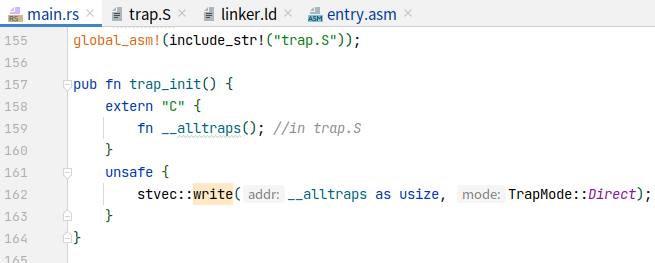
\includegraphics[width=0.8\linewidth]{os-trap-init}
    %        \caption{内核初始化}
    %    \end{figure}
\end{frame}


%------------------------------------------------
\begin{frame}
    \frametitle{kernel mode OS: 内核实现:系统调用处理框架}
    %	\framesubtitle{QEMU}
    %	\centering
    %	
\includegraphics[width=0.2\linewidth]{qemu}	
    进入trap\-handler前的硬件状态
    \begin{itemize}
        
    \item 发生异常的指令PC被存入sepc, 且PC被设置为stvec
    \item scause根据异常设置类型,stval被设置为出错的地址或者异常相关信息字
    \item 把sstatus CSR中的SIE置零,屏蔽中断,且SIE之前的值被保存在SPIE中
    \item 发生例外前的特权模式被保存在sstatus的SPP域,然后设置当前特权模式为S模式
        
    \end{itemize}	
    %    \begin{figure}
%    \centering
%    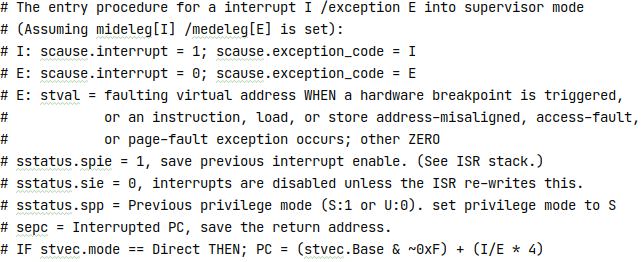
\includegraphics[width=0.9\linewidth]{rv-trap-begin}
    %        \caption{内核初始化}
    %    \end{figure}
\end{frame}

%------------------------------------------------
\begin{frame}
    \frametitle{kernel mode OS: 内核实现:系统调用处理框架}
    %	\framesubtitle{QEMU}
    %	\centering
    %	
\includegraphics[width=0.2\linewidth]{qemu}	
    
    \begin{itemize}
        
        \item 进入trap\-handler前的硬件状态
        
        
    \end{itemize}	
    %    \begin{figure}
    \centering
    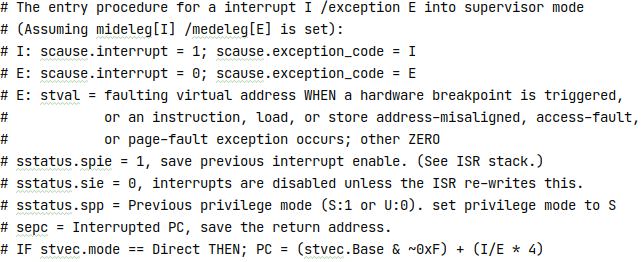
\includegraphics[width=0.9\linewidth]{rv-trap-begin}
    %        \caption{内核初始化}
    %    \end{figure}
\end{frame}

%------------------------------------------------
\begin{frame}
    \frametitle{kernel mode OS: 内核实现:系统调用处理框架}
    %	\framesubtitle{QEMU}
    %	\centering
    %	
\includegraphics[width=0.2\linewidth]{qemu}	
    trap\-handle处理框架
    \begin{itemize}
        
        \item 保存应用的中断上下文(trap\-context):\_\_alltraps
        \item 执行系统调用服务
        \item 恢复应用的中断上下文(trap\-context):\_\_restore
        \item sret返回到应用程序继续执行
    \end{itemize}	
    %    \begin{figure}
    \centering
    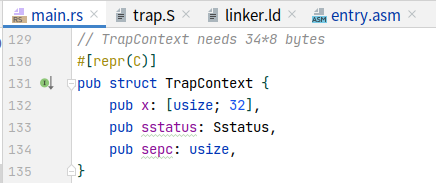
\includegraphics[width=0.6\linewidth]{os-trap-context}
    %        \caption{内核初始化}
    %    \end{figure}
\end{frame}

%------------------------------------------------
\begin{frame}
    \frametitle{kernel mode OS: 内核实现:系统调用处理框架}
    %	\framesubtitle{QEMU}
    %	\centering
    %	
\includegraphics[width=0.2\linewidth]{qemu}	
    trap\-handle处理框架
    \begin{itemize}
        \item sret返回到应用程序继续执行
    \end{itemize}	
    %    \begin{figure}
    \centering
    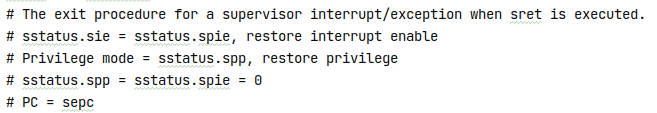
\includegraphics[width=1.0\linewidth]{os-trap-sret}
    %        \caption{内核初始化}
    %    \end{figure}
\end{frame}
%------------------------------------------------

%------------------------------------------------
\begin{frame}
    \frametitle{kernel mode OS: 内核实现:创建并初始化应用}
    %	\framesubtitle{QEMU}
    %	\centering
    %	
\includegraphics[width=0.2\linewidth]{qemu}	

    \begin{itemize}
        \item 模拟应用发出系统调用时的中断上下文
    \end{itemize}	
    %    \begin{figure}
    \centering
    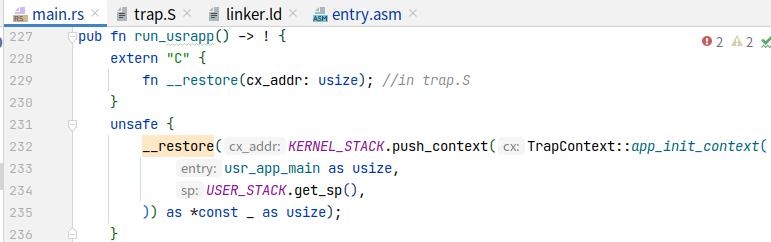
\includegraphics[width=1.0\linewidth]{os-run-app}
    %        \caption{内核初始化}
    %    \end{figure}
\end{frame}

%------------------------------------------------
\begin{frame}
    \frametitle{kernel mode OS: 内核实现:创建并初始化应用}
    %	\framesubtitle{QEMU}
    %	\centering
    %	
\includegraphics[width=0.2\linewidth]{qemu}	
    
    \begin{itemize}
        \item 初始化应用的中断上下文
    \end{itemize}	
    %    \begin{figure}
    \centering
    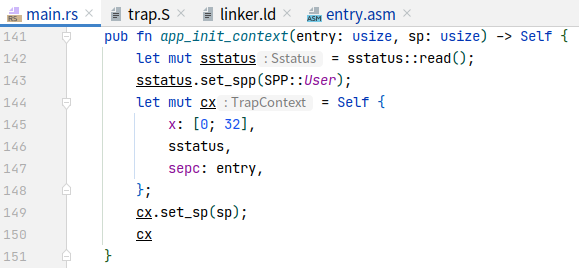
\includegraphics[width=0.9\linewidth]{os-init-app}
    %        \caption{内核初始化}
    %    \end{figure}
\end{frame}
%------------------------------------------------
%------------------------------------------------
\begin{frame}
    \frametitle{小结}
    \begin{itemize}
        \item 了解kernel-mode OS如何创建应用程序
        \item 了解kernel-mode OS如何让应用程序执行
        \item 了解应用程序如何得到kernel-mode OS的服务
        \item 读懂汇编代码的含义和功能
    \end{itemize}
\end{frame}
%------------------------------------------------
%
%
%\begin{frame}[plain]
%%	\frametitle{RISC-V CPU 启动过程--初始化CPU}
%	%	\framesubtitle{QEMU}
%	%	\centering
%%	
\includegraphics[width=0.1\linewidth]{qemu}	
%%	\begin{itemize}
%%		
%%		\item RISC-V CPU 启动过程--初始化CPU
%%		
%%	\end{itemize}		
%	\centering
%	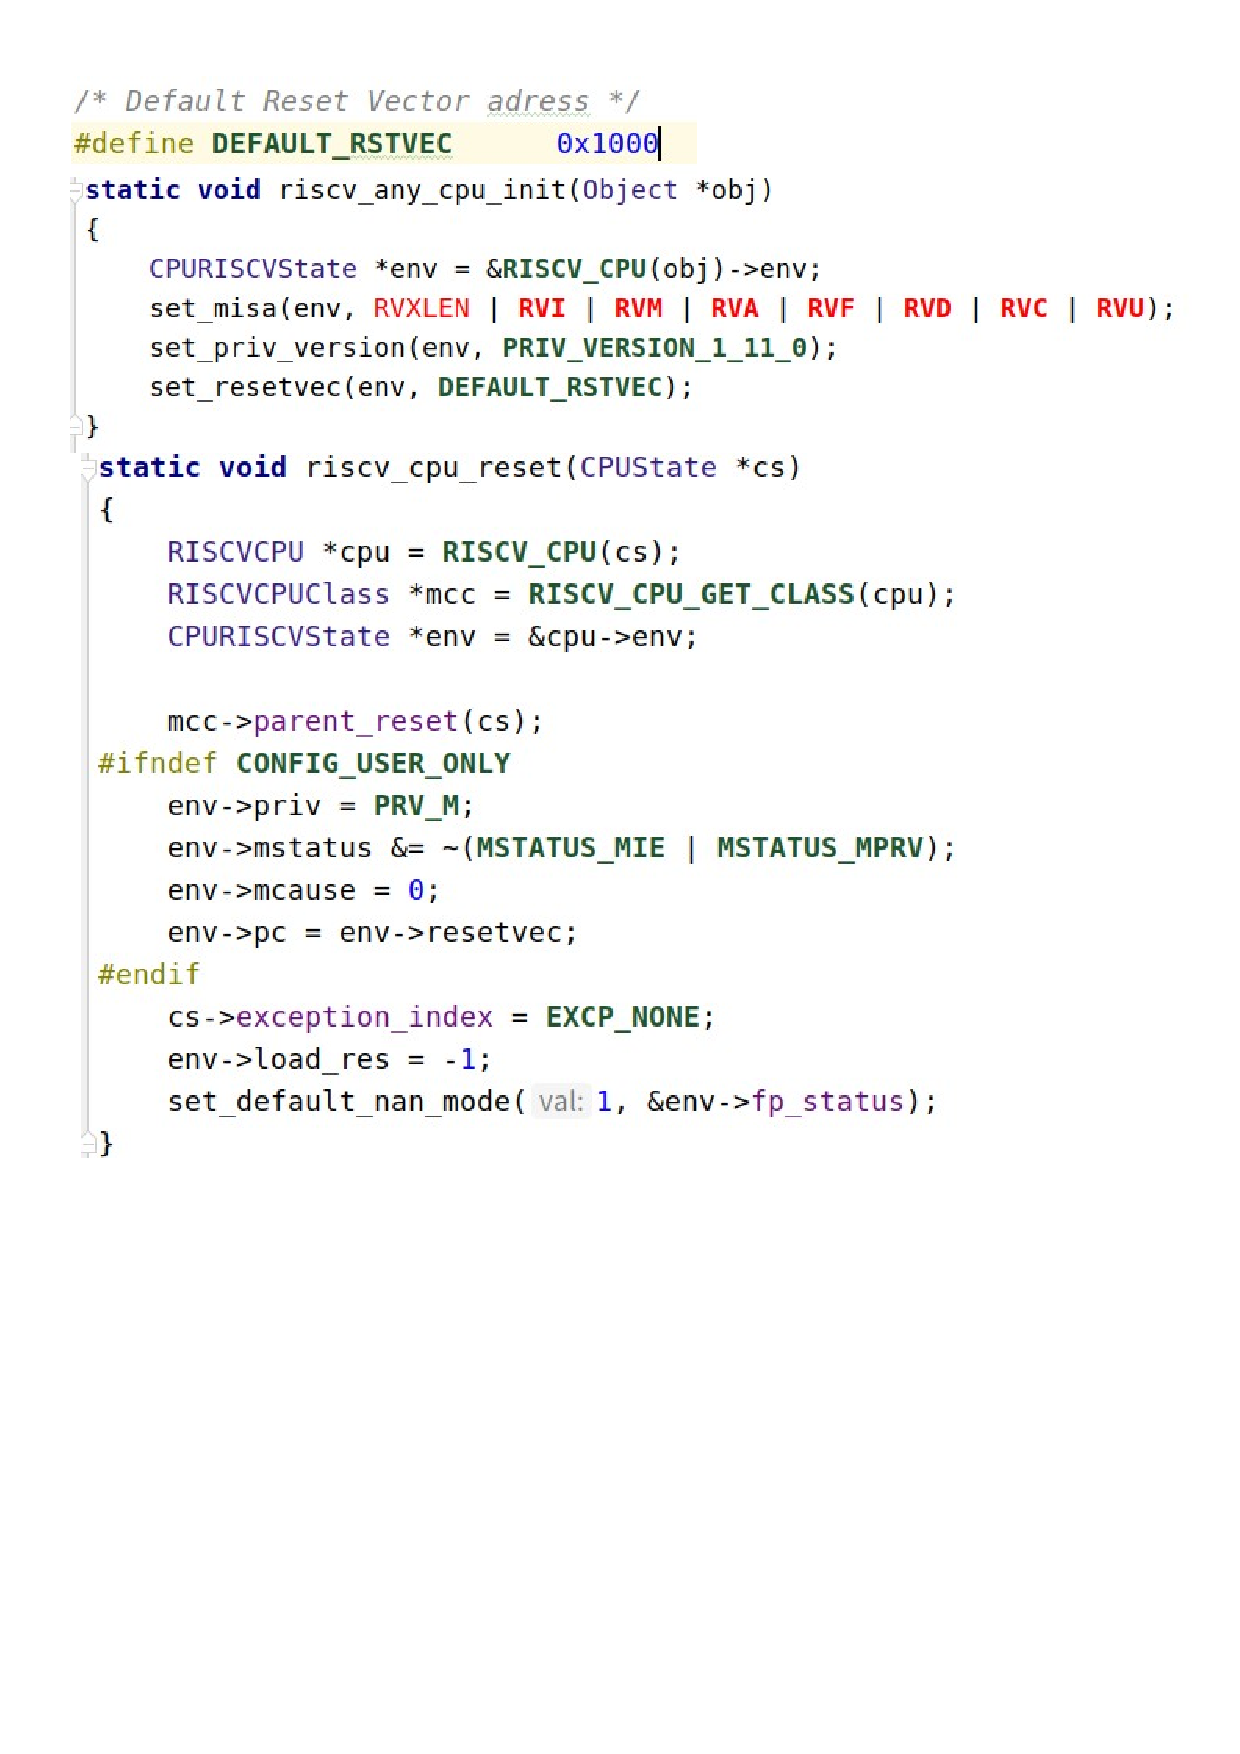
\includegraphics[width=0.65\linewidth]{qemu-initcpu}
%\end{frame}
%
%\begin{frame}
%	\frametitle{RISC-V CPU}
%	%	\framesubtitle{QEMU}
%%	\centering
%	
\includegraphics[width=0.1\linewidth]{qemu}	
%	\begin{itemize}
%		
%		\item RISC-V CPU 启动过程--初始化内存
%		
%	\end{itemize}	
%	
%	\centering
%	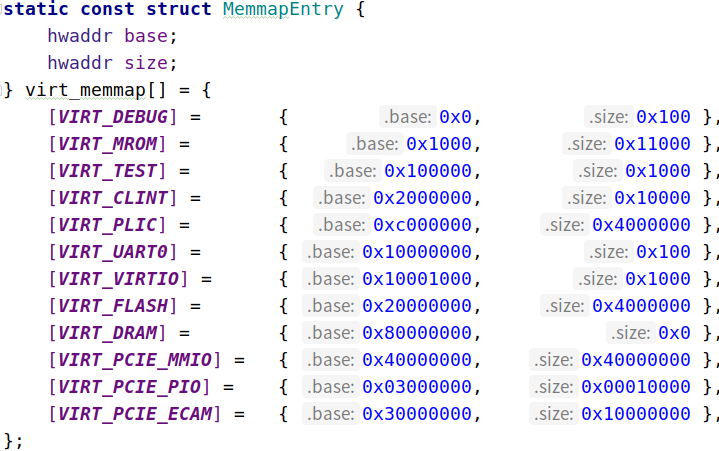
\includegraphics[width=0.6\linewidth]{qemu-initmem}
%\end{frame}
%
%\begin{frame}[plain]
%%	\frametitle{ RISC-V CPU 启动过程--初始化外设}
%	%	\framesubtitle{QEMU}
%	%	\centering
%	%	
\includegraphics[width=0.1\linewidth]{qemu}	
%%	\begin{itemize}
%%		
%%		\item RISC-V CPU 启动过程--初始化外设
%%		
%%	\end{itemize}	
%	\centering
%	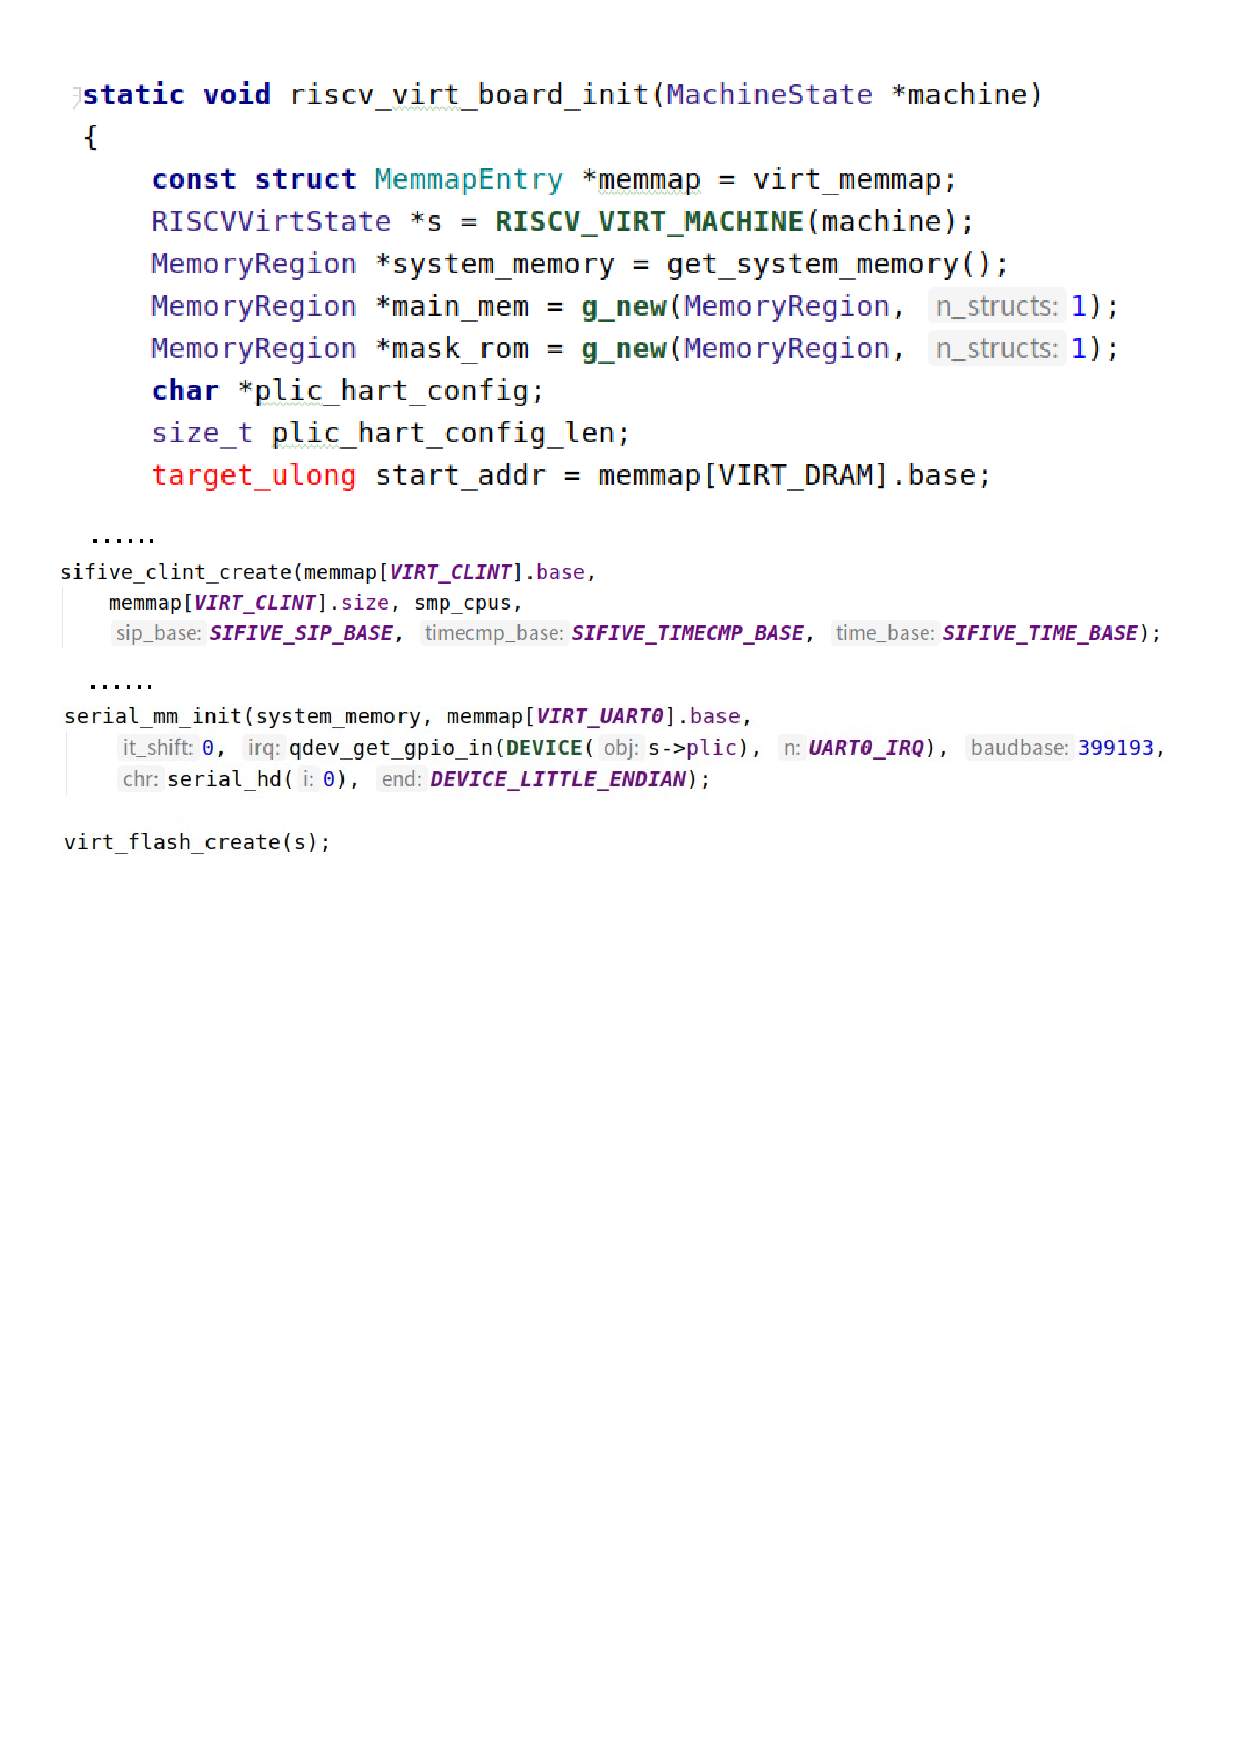
\includegraphics[width=0.8\textwidth]{qemu-initboard}
%\end{frame}
%
%
%\begin{frame}[plain]
%	\frametitle{RISC-V CPU 启动过程--ROM初始化代码}
%	%	\framesubtitle{QEMU}
%	%	\centering
%%	
\includegraphics[width=0.1\linewidth]{qemu}	
%%	\begin{itemize}
%%		
%%		\item RISC-V CPU 启动过程--ROM初始化代码
%%		
%%	\end{itemize}	
%	
%	\centering
%	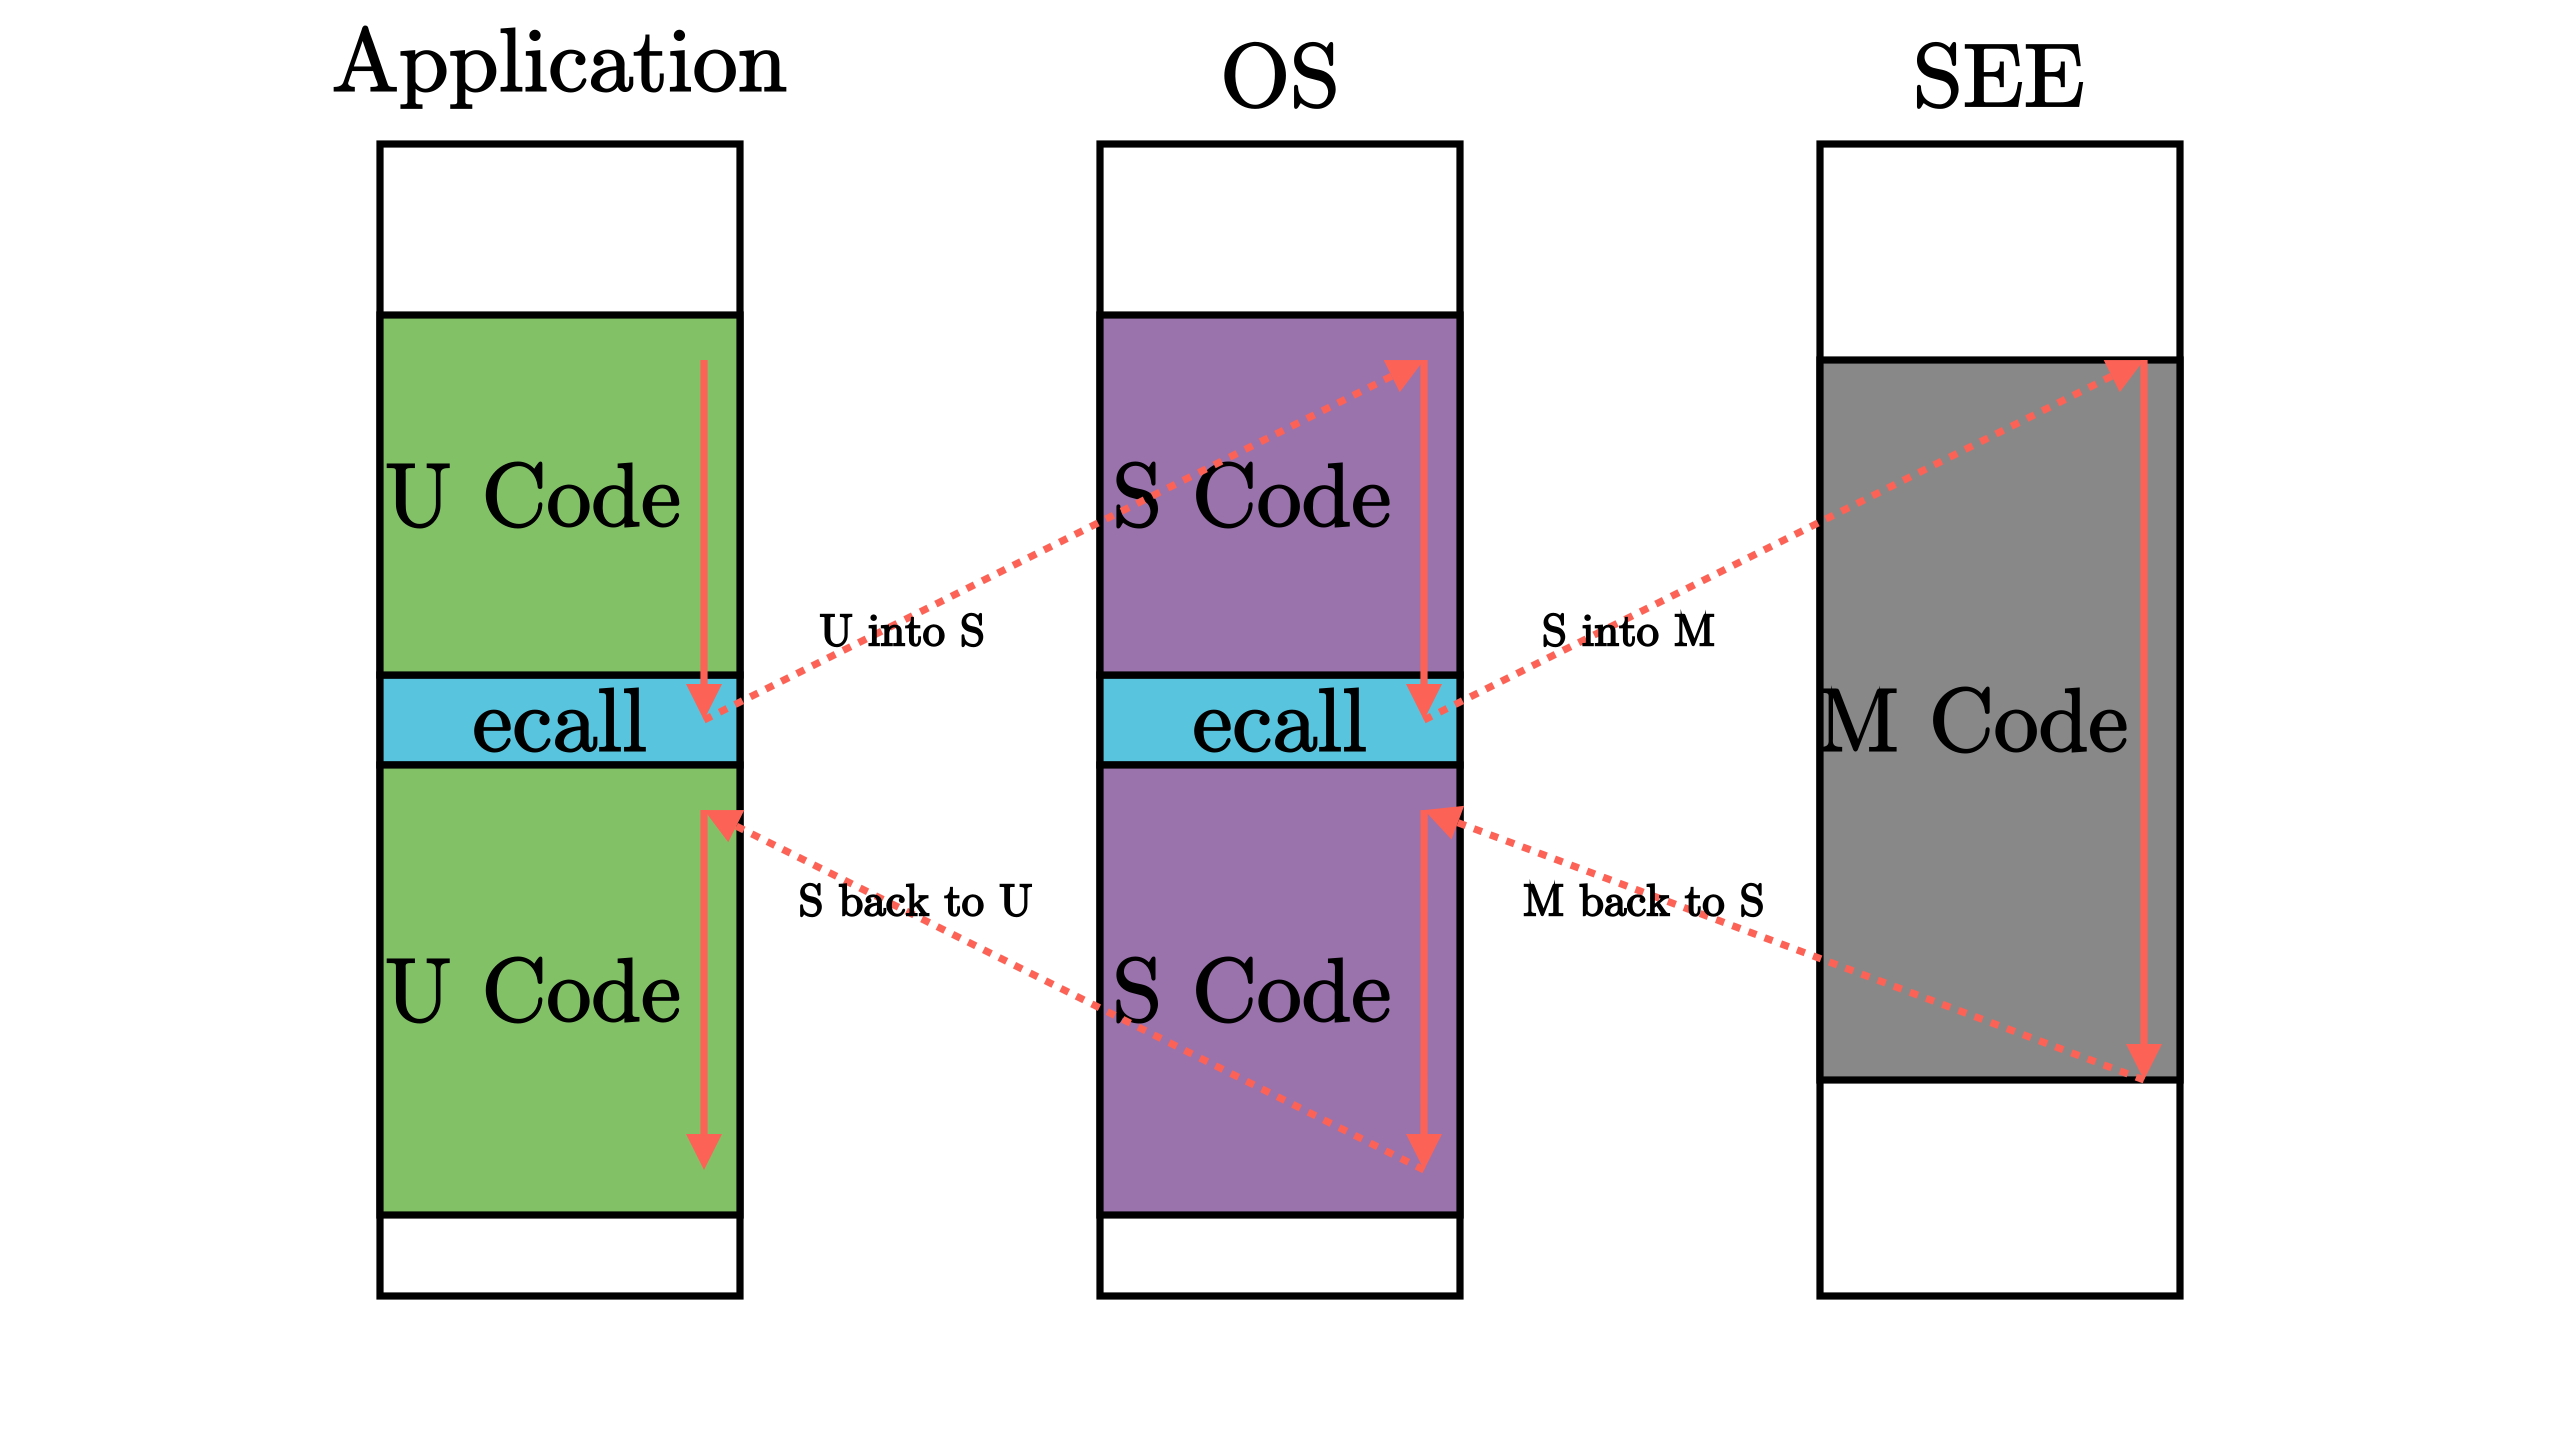
\includegraphics[width=0.8\linewidth]{EnvironmentCallFlow}
%\end{frame}


%----------------------------------------------------------------------------------------

\end{document}
